\chapter{The structural flexibility of \protein{Mad1} facilitates the coupling between \protein{Mad2}'s conformational change and the assembly of the mitotic checkpoint complex (MCC)}
\label{chpt:4}

In previous chapters, we presented evidence on the cooperativity among multiple MELT motifs on the same \protein{Knl1} phosphodomain (the first layer in the SAC signaling cascade). This phenomenon is probably explained by SAC proteins that concurrently bind to these MELT motifs in close spatial proximity (the second layer). In this chapter, we will focus on the spatio-temporal coupling scaffolded by \protein{Mad1} between \protein{Mad2}'s conformational change and the assembly of the MCC \cite{BUB1-CDC20-MAD1,Tripartite}. We term it ``the third layer'' in the SAC signaling cascade. % As mentioned in \myref{Chapter3Discussions}, \protein{Mad1} can be recruited to signaling kinetochores by multiple pathway.

The formation of the \protein{Cdc20}-\protein{Mad2} dimer, an MCC subcomplex, is considered to be the rate-limiting step in the assembly of the MCC based on an \Latin{in vitro} study \cite{Faesen2017}. However, how \protein{Cdc20}-\protein{Mad2} dimerization is catalyzed in the cell was unclear for a long time. Critical studies published later showed that locking cytosolic \protein{Mad2} to the closed conformation inhibited the dimerization between \protein{Cdc20} and \protein{Mad2} and compromised the SAC signaling activity \cite{Ma+Poon2016,Ma+Poon2018,Kim2018}. These findings hinted that the conformational change of \protein{Mad2} and \protein{Cdc20}-\protein{Mad2} dimerization might be temporally coupled. In 2021, two papers published back-to-back (based on either \Latin{in vitro} reconstitution \cite{BUB1-CDC20-MAD1} or studies in \Latin{C. elegans} \cite{Tripartite}) presented evidence supporting the cooperative binding of \protein{Cdc20} to signaling kinetochores and the spatio-temporal coupling between \protein{Mad2}'s conformational change and the formation of the \protein{Cdc20}-\protein{Mad2} dimer (see \myref{TwoModels}), which offered critical molecular insight into the synergy in this process.

In this chapter, we approached the suggested spatio-temporal coupling from a different angle -- by looking into the role of the conserved structural flexibility of \protein{Mad1} in the catalysis of \protein{Cdc20}-\protein{Mad2} dimerization. We began this hypothesis-driven study independently in 2018, which has evolved into a collaboration project. I am the sole contributor to most cell biology data here. \Latin{In vitro} reconstitution results from our collaborators (Dr. Valentina Piano from Dr. Andrea Musacchio's group at the Max Planck Institute of Molecular Physiology in Germany) will be mentioned to form a coherent story, but those data are not included here. % Simon Han performed preliminary tests on the internal tagging of Mad2p in the budding yeast.

\section{The molecular mechanism of \protein{Cdc20}-\protein{Mad2} dimerization: the ``Assembly Line'' model \Latin{versus} the ``Knitting'' model}
\label{TwoModels}

The formation of the \protein{Cdc20}-\protein{Mad2} dimer, an MCC subcomplex, is considered to be the rate-limiting step in the assembly of the MCC based on an \Latin{in vitro} study \cite{Faesen2017}. However, how \protein{Cdc20}-\protein{Mad2} dimerization is catalyzed in the cell was unclear for a long time. \protein{Cdc20} has a flexible N-terminal region with a \protein{Mad2}-interacting motif (MIM) and a C-terminal WD40 \textbeta{}-propeller fold \cite{hCDC20Structure} (in \myref{TwoModelCartoons}, the N- and C-terminal regions are represented by a light gray line and a light gray circle, respectively). \protein{Mad2} has three known conformations: the open conformation (denoted as O-\protein{Mad2} and illustrated as a magenta open lock with a circular body in \myref{TwoModelCartoons}), the intermediate conformation (denoted as I-\protein{Mad2} and illustrated as a peach open lock with a rectangular body in \myref{TwoModelCartoons}), and closed (denoted as C-\protein{Mad2} and illustrated as a red closed lock with a rectangular body in \myref{TwoModelCartoons}) \cite{I-MAD2}. A popular explanation of the catalytic mechanism of the switch of \protein{Mad2} from the open conformation to the closed conformation is the template model \cite{TemplateModel}. This model states that the conformational switch of \protein{Mad2} may be facilitated by the homodimerization between a closed \protein{Mad2} (bound to \protein{Mad1}'s MIM in the \protein{Mad1}-\protein{Mad2} heterotetramer) and the \protein{Mad2} that undergoes the conformational switch. C-\protein{Mad2} binds to \protein{Cdc20}, buckling the MIM of \protein{Cdc20} in a safety belt-like manner similar to how C-\protein{Mad2} binds to \protein{Mad1} \cite{Structure1GO4, SpMCC}. The \protein{Cdc20}-\protein{Mad2} dimer binds to \protein{BubR1}/\protein{BubR1}-\protein{Bub3} and forms the MCC.

\protein{Cdc20} binds to \protein{Mad1}'s C-terminal RING finger-containing proteins, WD repeat-containing proteins, and DEAD-like helicases (RWD) domain phosphorylated by \protein{Mps1} through an N-terminal basic motif of \protein{Cdc20} \cite{Ji2017eLife, BUB1-CDC20-MAD1} (illustrated in \myref{TwoModelCartoons} as the contact between \protein{Cdc20}'s light gray N-terminal region and \protein{Mad1}'s dark green C-terminal domain). Given the spatial proximity between the catalytic site of \protein{Mad2}'s conformational switch and the MIM of \protein{Cdc20}, it is attractive to investigate the potential coupling between \protein{Mad2}'s conformational switch (\textcircled{\small{1}} in \myref{TwoModelCartoons}) and the binding between \protein{Cdc20} and \protein{Mad2} (\textcircled{\small{2}} in \myref{TwoModelCartoons}). Therefore, we set out to test two opposite models, which we named the ``assembly line'' model and the ``knitting'' model. As the names suggest, the ``assembly line'' model indicates that the two processes happen in two separate steps and newly switched \protein{Mad2} from step \textcircled{\small{1}} enters a free cytosolic pool and then participates in step \textcircled{\small{2}}, as if two steps in an assembly line mediated by a warehouse. In contrast, the ``knitting'' model indicates that like knitting, the two processes are closely coordinated in one step  (\Latin{i.e.}, \textcircled{\small{1}} is coupled to \textcircled{\small{2}}). Metaphorically, the two structural regions of \protein{Mad1} shown in the top panel of \myref{HsMAD1CTerStructure} function as the two knitting needles.

\begin{figure}
    \centering
    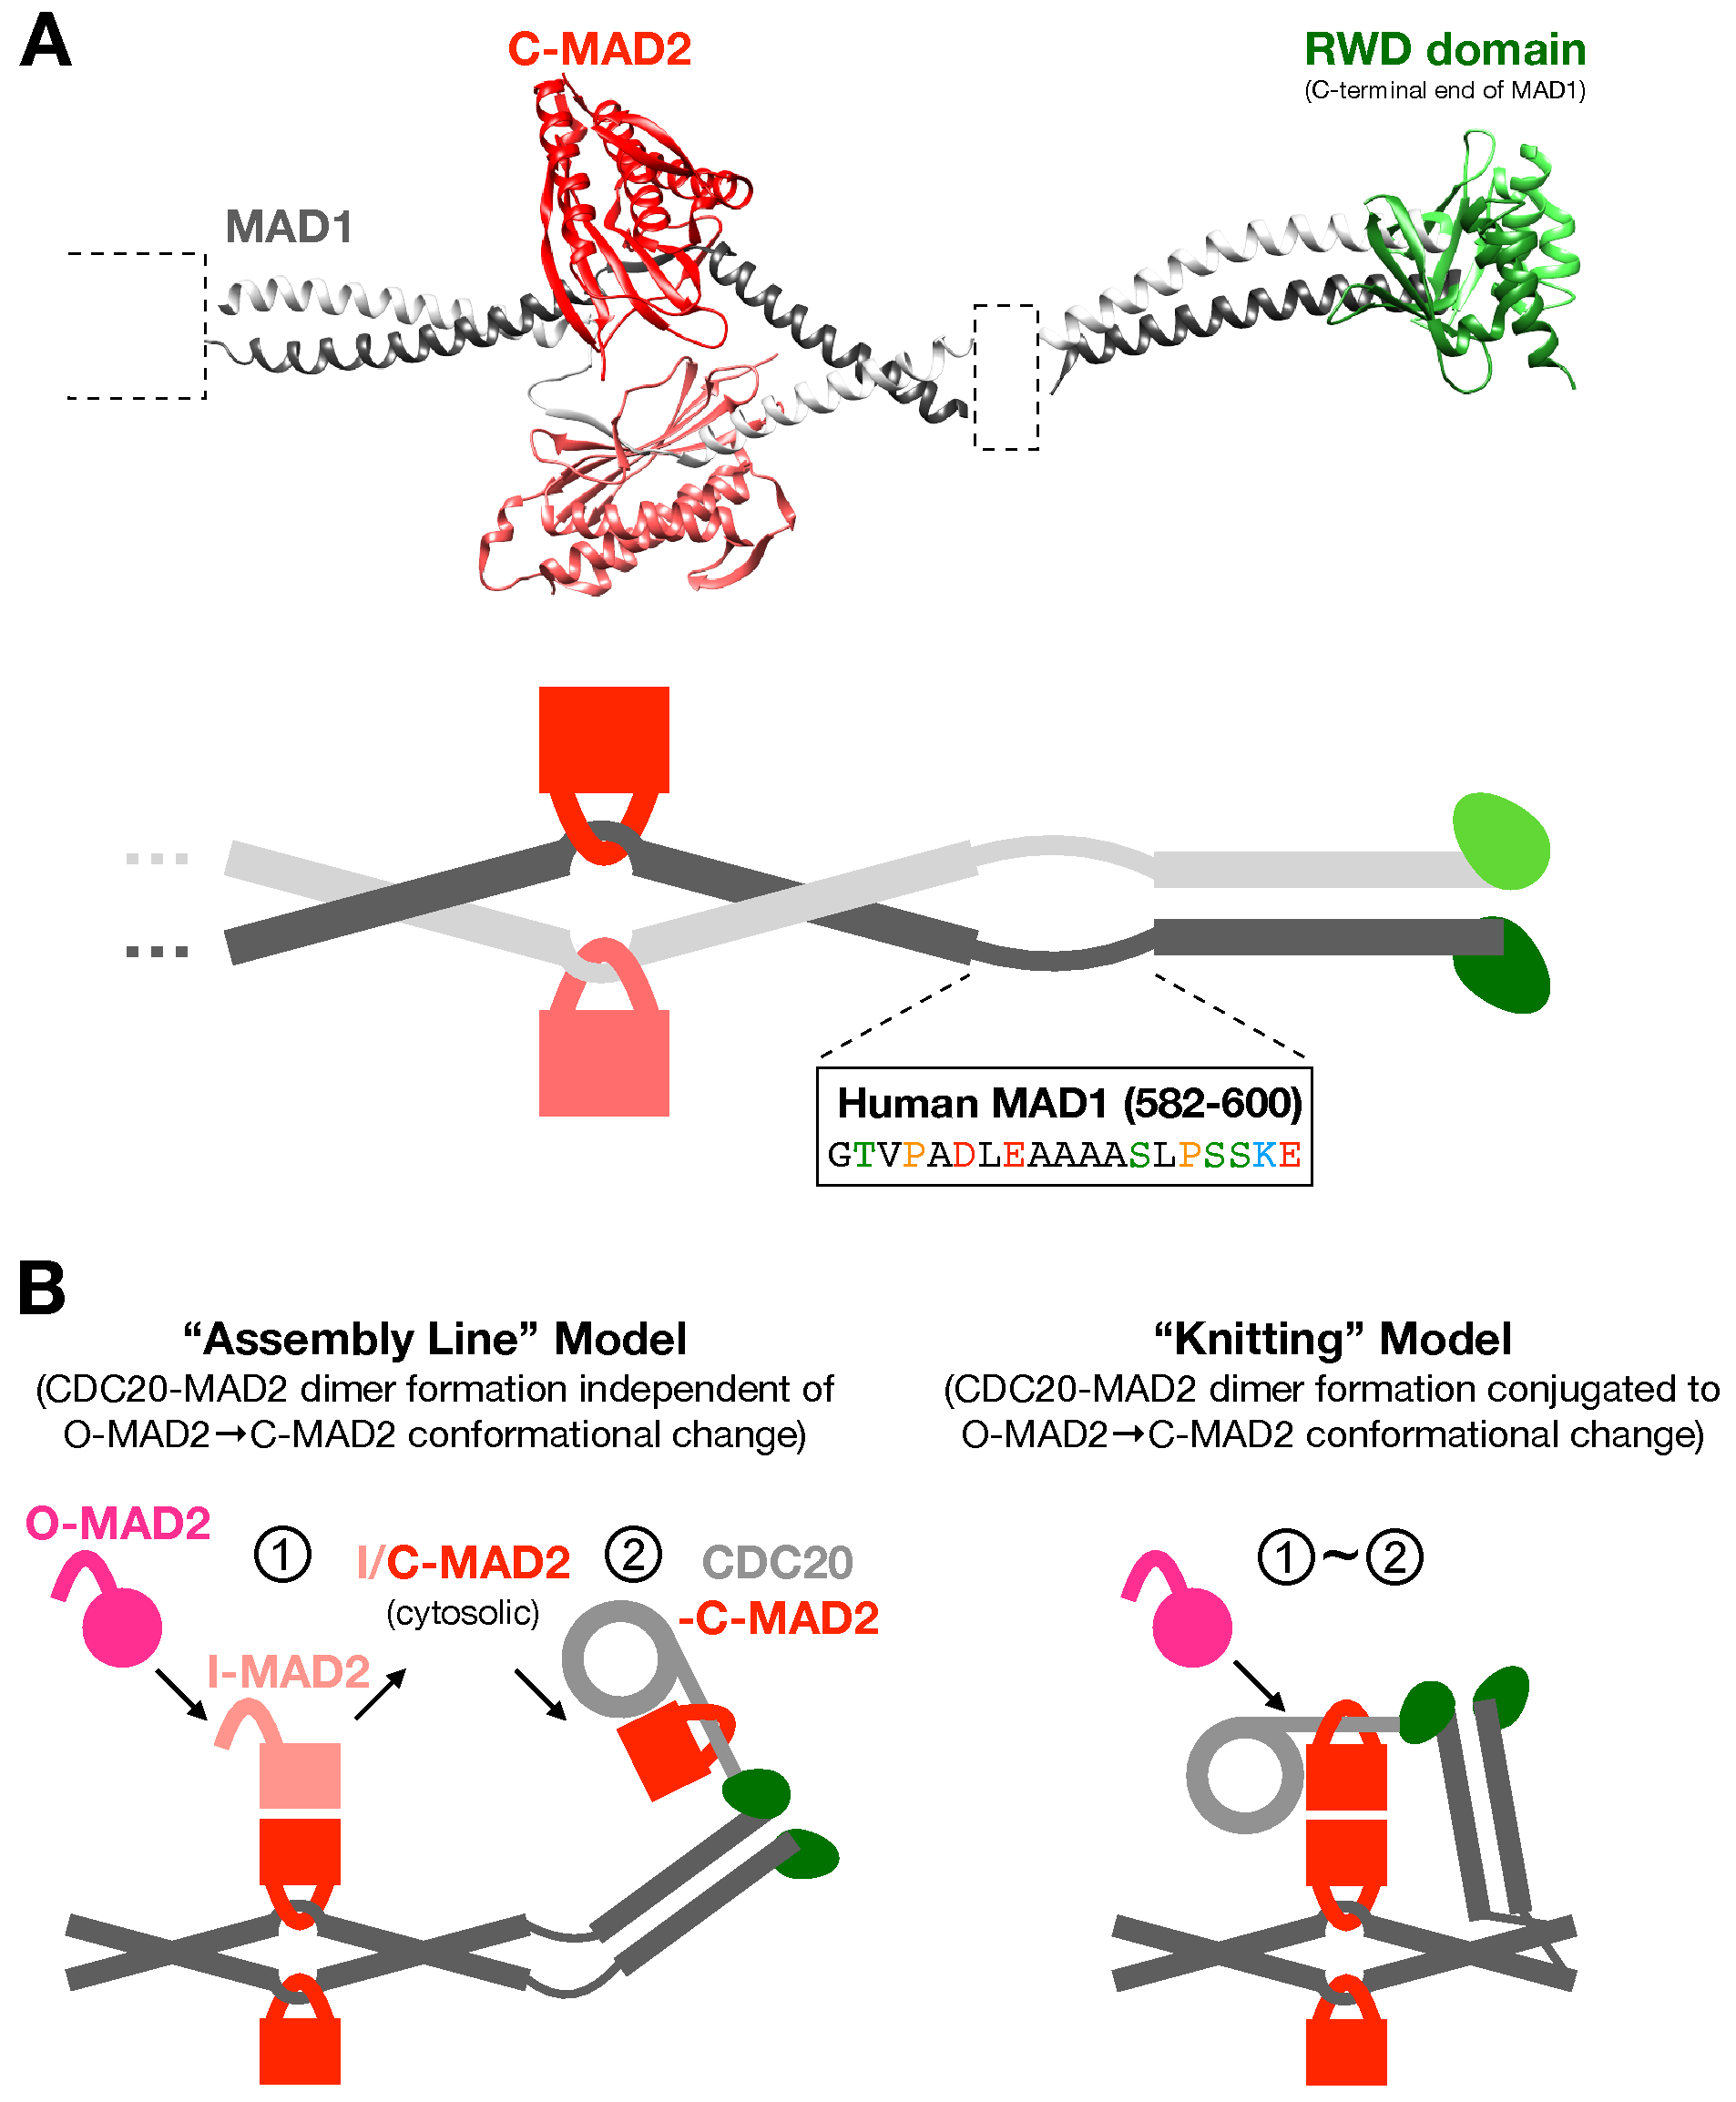
\includegraphics[width=0.78\textwidth]{chapters/figures/MAD1C+KnittingModel.pdf}
    \phantomsubfiglabel{HsMAD1CTerStructure} % subfigure A
    \phantomsubfiglabel{TwoModelCartoons} % subfigure B
    \caption{\textbf{The structure of the \protein{Mad1}-\protein{Mad2} heterotetramer and the two models of the molecular mechanism of \protein{Cdc20}-\protein{Mad2} dimerization.}}
    \noindent\justifying (A) Top panel: the known structure of the \protein{Mad1}-\protein{Mad2} heterotetramer. PDB IDs: 1GO4 (left, \cite{Structure1GO4}), 4DZO (right, \cite{Structure4DZO}). Structures of the N-terminus and the segment spanning a.a. 580--597 are unknown. Various secondary structure prediction algorithms consistently predicted this segment to be a flexible loop (though the predicted starting and ending positions may vary among different algorithms). Bottom panel: a cartoon illustrating the known structure of the \protein{Mad1}-\protein{Mad2} heterotetramer. The color scheme matches the top panel. To distinguish the two \protein{Mad1} proteins [and their C-terminal RWD domains] and the two \protein{Mad2} proteins, slightly different colors are applied. In all cartoons later, both copies will use the same color scheme. The sequence of the loop region (a.a. 582--600) predicted by COILS is shown \cite{LupasCOILS}. All cartoons in this chapter are not to scale. (B) The two models of the molecular mechanism of \protein{Cdc20}-\protein{Mad2} dimerization: the "assembly line" model (left) and the "knitting" model (right).
    \label{MAD1C+KnittingModel}
\end{figure}

We reason that the ``knitting'' model is more realistic based on many pieces of evidence from previous literature. First, locking cytosolic \protein{Mad2} to its closed conformation inhibited the dimerization between \protein{Cdc20} and \protein{Mad2} and compromised the SAC signaling activity \cite{Ma+Poon2016, Ma+Poon2018, Kim2018}, which can be interpreted by the ``knitting'' model. Second, the binding of \protein{Cdc20} to \protein{Mad1}'s RWD domain is suggested to be important to the SAC signaling activity \cite{Kruse2014, SpMad1, Faesen2017, Ji2017eLife}. One explanation is that the binding may increase the local concentration of \protein{Cdc20}, which is better harnessed by the ``knitting'' model. The anchoring of the basic motif of \protein{Cdc20} to \protein{Mad1}'s RWD domain may even topologically hinder the stringing of \protein{Mad2} that is already in the closed conformation because \protein{Cdc20}'s MIM is between the basic motif and the \textbeta{}-propeller. Third, two recent studies strongly supported the spatio-temporal coupling between \protein{Mad2}'s conformational change and the formation of the \protein{Cdc20}-\protein{Mad2} dimer \cite{BUB1-CDC20-MAD1, Tripartite}.

In this chapter, we intend to prove the "knitting" model by introducing mutations to \protein{Mad1} that theoretically only impair the SAC signaling activity if the "knitting" model is correct. It should be noted that there is a gray area between the two models, given that I-\protein{Mad2} can exist in the solution \cite{I-MAD2}, which may be the fresh \protein{Mad2} conformer coming off the template-based conformational switch, entering the cytosolic pool, and eventually binding to \protein{Cdc20} (becoming C-\protein{Mad2} thereafter). We categorize this situation into the "assembly line" model (also illustrated in \myref{TwoModelCartoons}) because our mutational approach should not impair the SAC signaling activity in this case either (see \myref{LoopDeletionSection}).

\section{The primary sequence of \protein{Mad1}'s loop region is not conserved but the secondary structure is}
% To understand which model is correct/design an experiment to prove which hypothesis is correct in a more direct way (or at least from a different angle), we need to understand the structure of MAD1 first.

\section{The \protein{Mad1}-\protein{Mad2} heterotetramer may adopt a fold-back conformation both \Latin{in vivo} and \Latin{in vitro}}
% 13 nm

\section{\protein{Mad1}'s loop region is important to the SAC signaling activity \Latin{in vivo}}
\label{LoopDeletionSection}

\section{The function of \protein{Mad1}'s loop region does not depend on the potential phosphorylation of any serine or threonine residues within it}

\section{The structural flexibility of \protein{Mad1} enabled by its loop region facilitates the ``knitting'' of the MCC}
\label{FinalKnittingModel}

\section{Discussions}
\label{Chapter4Discussions}

In this study, we showed for the first time that the \protein{Mad1}-\protein{Mad2} heterotetramer can assume a fold-back conformation both \Latin{in vitro} and \Latin{in vivo}. Our preliminary data indicate that the structural flexibility is enabled by a flexible loop in the C-terminus of \protein{Mad1}, whose secondary structure is conserved. This loop region is important to the SAC signaling activity both \Latin{in vitro} and \Latin{in vivo} and its role does not depend on any potential phospho-regulation of the serine/threonine residues within. We proposed a ``knitting'' model to explain how the structural flexibility of \protein{Mad1}-\protein{Mad2} heterotetramer may facilitate the spatio-temporal coupling between \protein{Mad2}'s conformational change and \protein{Cdc20}-\protein{Mad2} dimerization. It should be noted that even in the absence of \protein{Cdc20}, O-\protein{Mad2} can bind to the \protein{Mad1}-\protein{Mad2} heterotetramer, complete the conformational switch, and dissociate as C-\protein{Mad2} \Latin{in vitro} \cite{Yang2008}. Finding out whether \protein{Cdc20} increases the rate of \protein{Mad2}'s conformational switch will help us further understand the mechanism of the catalysis.

\protein{Mad1} has a long half-life under normal conditions \cite{MAD1MAD2Half-life}. And like \protein{Bub1} \cite{Raaijmakers2018, RZZ-MAD1vsBUB1-MAD1_2018, siROD_Zhang2019}, even a small pool of \protein{Mad1} (at less than 10\% of its physiological concentration in our knockdown experiments) can maintain a considerable level of SAC signaling activity in nocodazole-treated cells. Future studies should consider combining RNA interference (or induced knockout of \gene{Mad1}) with induced acute degradation of \protein{Mad1} proteins to reduce the contribution of the remaining endogenous \protein{Mad1} homodimer to the SAC signaling activity and to minimize the chance of heterodimerization between the remaining endogenous \protein{Mad1} and the rescuing \protein{Mad1} variants in such knockdown-rescue experiments. %(AID, Trim-Away, etc. for such a nuclear protein during the interphase/prophase).

Given the critical role of \protein{Mad1}'s structural flexibility enabled by its loop region, it would be interesting to replace the flexible loop with a turn to lock \protein{Mad1} in the fold-back conformation and see how the SAC signaling activity is affected. Another way to advance our understanding is to investigate whether the two pools of \protein{Mad1} (adopting either the fold-back or extended conformation) inter-convert at a physiologically meaningful rate in the cell using single-molecular approaches. Even though the two proline residues (P585 and P596) in \protein{Mad1}’s loop region may be important to the SAC signaling activity \Latin{in vivo}, no \protein{Mad1}-interacting protein with either FK506-binding or peptidylprolyl cis-trans isomerase activity has been identified in the PrePPI database using the gene ontology enrichment analysis as of March 2022 \cite{PrePPI}. Additionally, it might be worth finding out whether the equilibrium between the two conformations in the cell is the same as purified \protein{Mad1}-\protein{Mad2} heterotetramer \Latin{in vitro}, which would tell us if the conformation distribution is under active regulation in the cell that costs energy \cite{MAD2Dynamics}. % However, this does not completely rule out the possibility because the interaction between \protein{Mad1} and a peptidylprolyl isomerase might be transient.

Two missense variants (D587N and A593V) related to \protein{Mad1}’s loop region were recorded in the Genomic Data Commons Data Portal as of March 2022 \cite{GDC}, but the impact of both point mutations is predicted to be benign. Therefore, the physiological impact of potential mutations in \protein{Mad1}’s loop region at the organism level is unclear. It would be interesting to see the physiological impact of introducing point mutations (for example, the multiple proline residues) in \protein{Mad1}’s loop region in various model systems.

In addition to \protein{Cdc20}, closed \protein{Mad2} also interacts with many other proteins (including \protein{Mad1}, \protein{Sgo2} \cite{SGO2-MAD2}, the insulin receptor \cite{MCC_IREndocytosis}, and \protein{Kif20a} \cite{KIF20A-MAD2}), likely by a similar ``safety belt'' mechanism \cite{Structure1GO4}. One question that comes up naturally is whether the same catalytic mechanism (the spatio-temporal coupling between \protein{Mad2}'s conformational change and \protein{Cdc20}-\protein{Mad2} dimerization) similarly applies to how \protein{Mad2} binds to other proteins (or even more generally, whether the same catalytic mechanism applies to how other HORMA domain proteins bind to other proteins \cite{HORMAReview})? One interesting finding is that the S214A mutation in human \protein{Mad1} impairs the homodimerization of \protein{Mad1} as well as the interaction between \protein{Mad1} and \protein{Mad2} \cite{ATMPhosphorylatesMad1S214}. S214A is unlikely to affect the binding of \protein{Mad2} to \protein{Mad1}'s MIM directly, given the structure of the \protein{Mad1}-\protein{Mad2} heterotetramer \cite{Structure1GO4} and the fact that S214 and MIM are over 300 amino acids apart. This suggested that the homodimerization of \protein{Mad1} might facilitate the binding of \protein{Mad2} to \protein{Mad1}. One possibility is that one copy of \protein{Mad1} may trans-activate the binding of \protein{Mad2} to the other copy of \protein{Mad1} in the \protein{Mad1}-\protein{Mad2} heterotetramer. Future experiments are needed to elucidate the structural and catalytic basis of how \protein{Mad2} ``buckles up'' its binding partners, which may unveil how \protein{Mad2} regulates mitosis beyond the assembly of the MCC \cite{Separase-SGO2-MAD2, KIF20A-MAD2}.

\Latin{In vitro} data from our collaborator (Dr. Valentina Piano at the MPI of Molecular Physiology in Germany) suggest that the critical role of the flexibility of \protein{Mad1} in scaffolding the spatio-temporal coupling between \protein{Mad2}'s conformational change and \protein{Cdc20}-\protein{Mad2} dimerization relies on \protein{Bub1} (data not shown). However, it is known that the assembly of the MCC also occurs during the interphase and prophase \cite{PremitoticMCC}. There has been no report on \protein{Bub1}'s localization at the NPC where the \protein{Mad1}-\protein{Mad2} heterotetramer is predominantly localized during the interphase and prophase. Therefore, either the flexibility of \protein{Mad1} alone scaffolds the coupling at the NPC or there may be a nucleoporin that functions similarly to \protein{Bub1}. Interestingly, the nuclear basket protein \protein{Tpr}, which directly associates with the \protein{Mad1}-\protein{Mad2} heterotetramer during the interphase and prophase \cite{TPR-MAD1_Lee2008}, is predicted to bind to \protein{Cdc20} directly in the PrePPI database \cite{PrePPI} (but we did not identify any ABBA motif on \protein{Tpr} which may potentially mediate the binding \cite{ABBA}). Future studies should look further into how the \protein{Mad1}-\protein{Mad2} heterotetramer may catalyze the formation of the \protein{Cdc20}-\protein{Mad2} dimer at the NPC during the interphase and prophase.

\section{Materials and Methods}
For methods of cell culture and Cre-\bacterialgene{lox} RMCE, see \myref{CellCulture+RMCE_Methods}. 

% MAD2^mSI editing

% FLIM

% The siRNAs targeting the 3'-UTR of \gene{Mad1} are from \cite{siMAD1-3UTR}.

% IXN

% Immunoblotting